% TikZ overlay on the real docx Figure 3 (Task 4a): fills the blank boxes.
\begin{tikzpicture}
\node[anchor=south west,inner sep=0] (img) at (0,0)
  {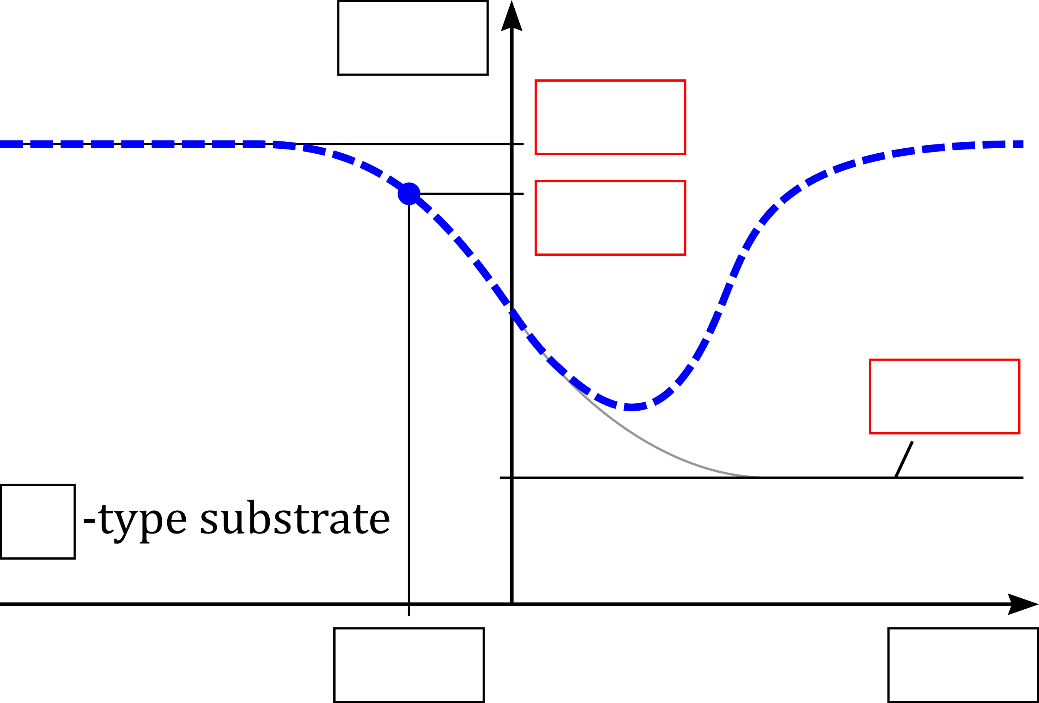
\includegraphics[width=0.66\textwidth]{figures/cv_fig3_blank.png}};
\begin{scope}[x={(img.south east)},y={(img.north west)}]
  \node at (0.385,0.955) {\small $C'$};
  \node at (0.585,0.840) {\scriptsize $C'_{\max}\!=\!C_{ox}$};
  \node at (0.585,0.695) {\scriptsize $C'_{FB}$};
  \node at (0.905,0.445) {\scriptsize $C'_{\min}$};
  \node at (0.035,0.280) {\small $p$};
  \node at (0.385,0.060) {\small $V_{FB}$};
  \node at (0.915,0.060) {\small $V_G$};
\end{scope}
\end{tikzpicture}
